\documentclass[times, utf8, seminar]{fer}
\usepackage{booktabs}
\usepackage{pdfpages}
\usepackage{listings}
\usepackage{mathtools}
\usepackage{algorithmic}
\usepackage{algorithm}
\usepackage{amsmath}
\usepackage{relsize}
\usepackage[colorinlistoftodos,prependcaption,textsize=tiny]{todonotes}

\renewcommand{\lstlistingname}{Isječak}
\DeclareMathOperator*{\argmax}{arg\,max}

\begin{document}

\lstset{
    basicstyle=\linespread{1.2}\ttfamily\footnotesize,
    keepspaces=true,
    numbers=left,
    frame=single,
    showspaces=false,
    numberstyle=\ttfamily,
    columns=flexible,
    extendedchars=true,
    inputencoding=utf8,
    literate={®}{{\textregistered}}1,
}

\voditelj{prof. dr. sc. Domagoj Jakobović}

\title{
    Sustavi za upravljanje heterogenom flotom ljudi i robota u logističkim centrima
}

\author{Herman Zvonimir Došilović}

\maketitle

\tableofcontents

\chapter{Uvod}
Logistički centri su dinamički i stohastički logistički sustavi
čija je temeljna zadaća prostornovremenska transformacija
dobara koja se odvija u procesima: (1) transporta, pregrupiranja i skladištenja gdje
su bitni procesi tokova dobara; (2) pakiranja i signiranja gdje su bitni procesi
pomaganja tokovima dobara; (3) dostavljanja i obrada naloga gdje su bitni procesi
tijekova informacija \citep{Paladin, buntak2012medjusobni}.

Razvojem informacijskih tehnologija elektroničko trgovanje \engl{ecommerce}
 posljednjih je godina
doživjelo veliki zamah u razvoju i poslovanju. Međutim, sa sve većim brojem narudžbi,
logistički procesi elektroničkog trgovanja postaju usko grlo
za ispunjenje narudžbi i njihovih rokova. Također, logistički procesi mogu uzrokovati
probleme poput sporih, neispravnih, izgubljenih, oštećenih i pogrešnih isporuka.
Pored toga, cijena logističkog procesa može iznositi
i do 40\% cijene korisnikove narudžbe.
Automatizacija logističkih procesa nudi poboljšanja učinkovitosti, smanjenje troškova
i smanjenje vremena posluživanja. Međutim, velika raznolikost i promjenljivost
narudžbi čini implementaciju automatizacije teškom. U obzir treba uzeti
ne samo tip i količinu neke naručene robe, nego i njihovu veličinu, njihov
oblik, masu, pa čak i svojstva i posebnosti pakiranja. Također, jednom
uspostavljeni automatizirani proces mora se moći lako prilagoditi
raznim promjenama u logističkom centru. To znači da se automatizirani sustavi
moraju lako skalirati i da moraju biti fleksibilni u svakom trenutku.
Kada govorimo o automatizaciji logističkih procesa elektroničkih trgovina, onda
razlikujemo automatizaciju protoka informacija i automatizaciju protoka robe.
Robotika nudi rješenje u automatiziranju protoka robe i roboti danas uspješno
ostvaruju zadatke koji se ponavljaju na fiksnim pozicijama sa željenom brzinom,
preciznosti i tereta. Robotika, također, nudi rješenje koje će
poboljšati učinkovitost, skalabilnost i fleksibilnost logističkih procesa.
Mobilni roboti omogućuju automatizirano izvršavanje zadataka na pozicijama
koje nisu više fiksne, međutim, tada je potrebno uskladiti suradnju između robota
i ljudi \citep{huang2015robotics}.

\pagebreak

Ovaj seminarski rad predstavit će i definirat će jedan stvarni problem koji
se pojavljuje uvođenjem mobilnih i autonomnih robota u logističke centre kako bi se
optimirala jedna faza logističkog procesa koja uključuje prikupljanje
artikala narudžbe, a odnosi se na upravljanje heterogenom flotom ljudi i robota.
Osim toga, napravit će se pregled područja i
metoda koje rješavaju sličan problem.

\chapter{Formalan opis problema raspoređivanja heterogene flote}
\label{chap:opis}
Heterogena flota ljudi i robota djeluje u skladištu logističkog centra i sastoji
se od ljudi i autonomnih mobilnih robota \engl{Autonomous Mobile Robots} koji se
mogu samostalno kretati i izbjegavati prepreke u dinamičnom okruženju. Roboti
također mogu preuzimati i odlagati teret na posebne paletne pozicije koje
paletu odvajaju od tla kako bi robot mogao spustiti odnosno podignuti paletu.
Slika \ref{fig:robot-01} prikazuje primjer takvog robota hrvatske tvrtke Gideon Brothers.
Na slici \ref{fig:robot-01} je također prikazana paletna pozicija na kojoj se nalazi
paleta s teretom.

\begin{figure}[htb]
    \centering
    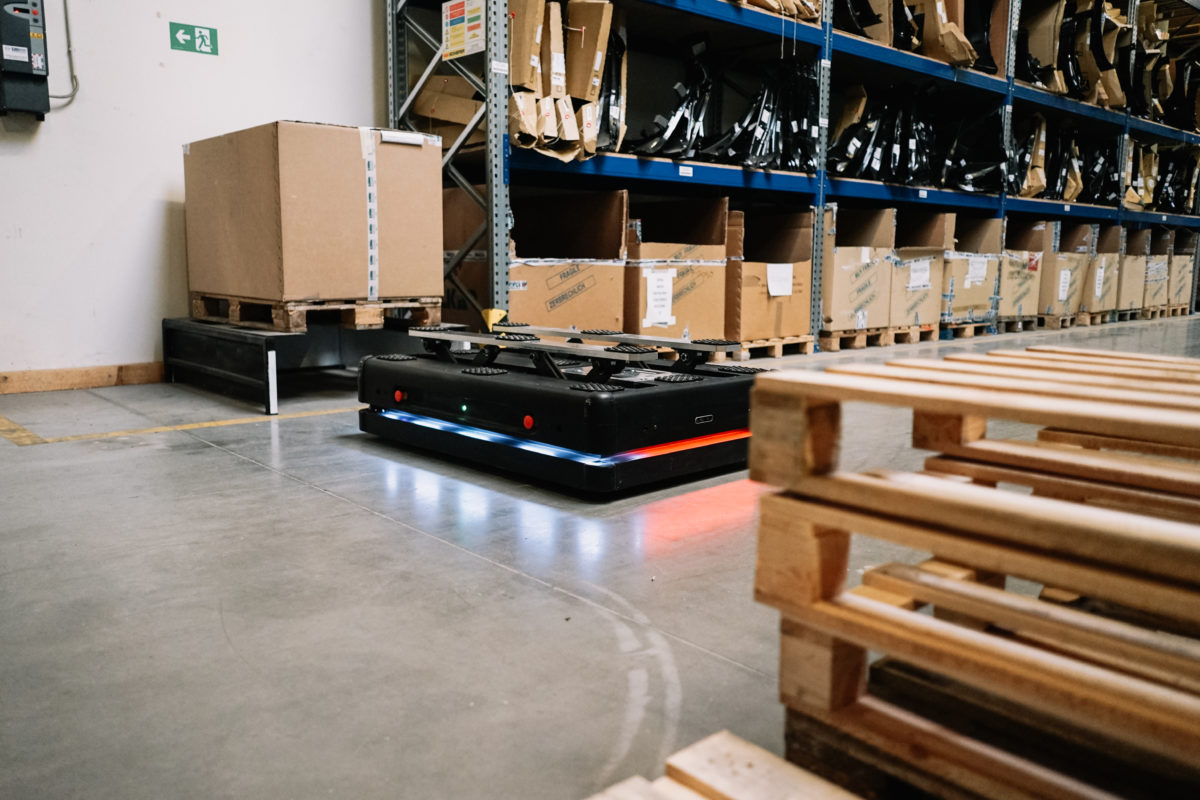
\includegraphics[height=9cm]{images/robot-01.jpg}
    \caption{Autonomni mobilni robot hrvatske tvrtke Gideon Brothers \citep{Gideon:Logisticsrobotlingo}.}
    \label{fig:robot-01}
\end{figure}

\pagebreak

U sustav za upravljanje heterogenom flotom ljudi i robota
(u daljnjem tekstu: \emph{Sustav}) narudžbe dolaze stohastički iz
sustava za upravljanje skladištem \engl{Warehouse Management System}.
Svaka narudžba sadrži više artikala i za svaki artikl poznata je njegova lokacija u skladištu.
Sustav \emph{WMS} također određuje kojim redoslijedom je potrebno prikupiti artikle kako bi
se narudžba izvršila.

Na početku svoga rada, robot odlazi do jedne od pozicija za preuzimanje praznih
paleta. Nakon što je preuzeo praznu paletu (slika \ref{fig:robot-02}), robot može započeti prikupljanje artikala (unaprijed
određenim redoslijedom) samo jedne narudžbe.
Kada robot dođe do pozicije na kojoj se nalazi artikl, čovjek stavlja taj artikl na robota.
Ljudi poslužuju robote, a roboti izvršavaju narudžbe. Jedan čovjek može posluživati više robota,
međutim, ne istovremeno.
Kada
je prikupio sve artikle koji pripadaju narudžbi, robot odlazi do jedne od pozicija za odlaganje punih paleta i
tamo odlaže paletu. Nakon odlaganja pune palete, smatra se da je robot izvršio narudžbu i da
je spreman za izvršavanje nove nakon što ponovo preuzme praznu paletu na jednoj od za to predviđenih
pozicija.

\begin{figure}[htb]
    \centering
    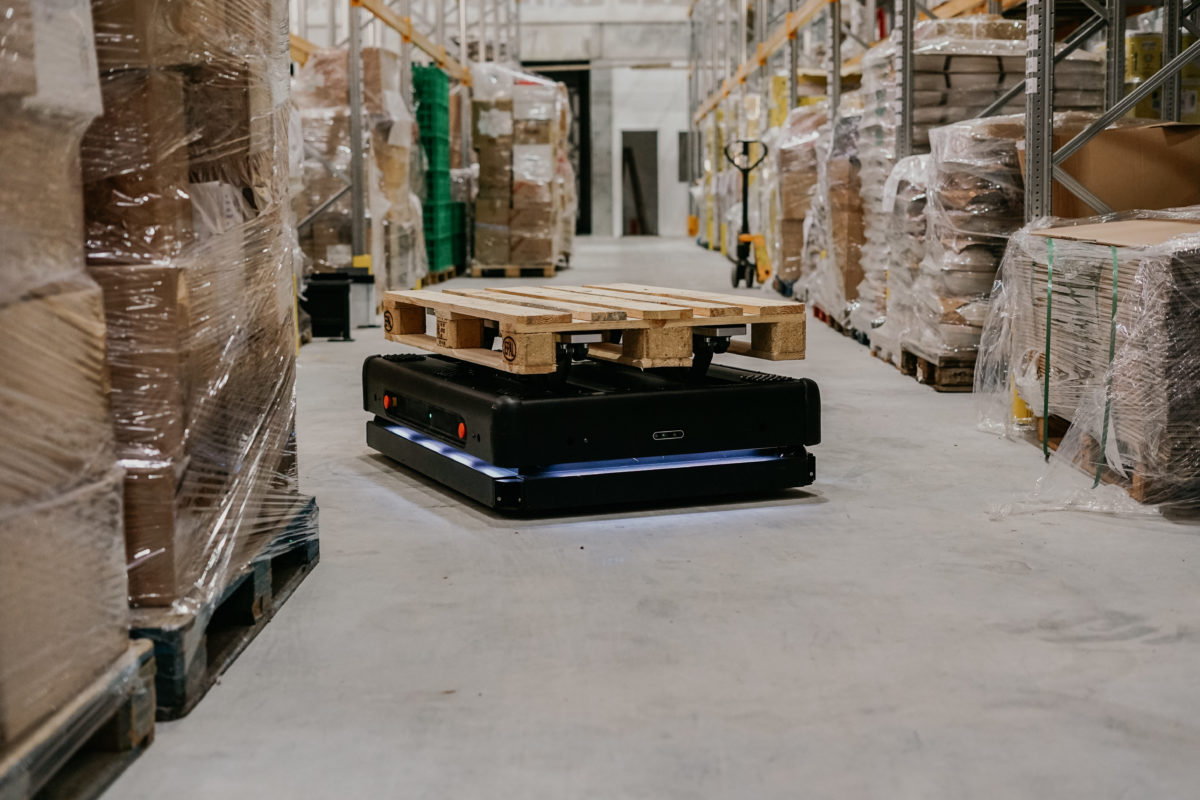
\includegraphics[height=9cm]{images/robot-02.jpg}
    \caption{Robot s praznom paletom, koji može započeti izvršavati narudžbu. \citep{Gideon:PollDebunks}}
    \label{fig:robot-02}
\end{figure}

Prvi zadatak sustava je da odredi koji robot će izvršiti koju narudžbu.
Drugi zadatak sustava je da odredi koji čovjek će poslužiti kojeg robota
i za koji artikl.
Teža inačica ovog problema uključuje i određivanje redoslijeda kojim je potrebno pokupiti
artikle pojedine narudžbe. Formalan opis stanja skladišta i ulaz u sustav bit će takav da će
sadržiti sve potrebne informacije kako bi se mogla riješiti i ova teža inačica problema.

\section{Definicija heterogene flote i skladišta}

Heterogena flota sastoji se od $N_p$ ($1 \le N_p \le 25$) ljudi i
 $N_r$ ($1 \le N_r \le 50$) robota,
koji se mogu kretati u po skladištu širine $W$ ($W \in \mathbb{N},\ 1 \le W \le 4500$)
i  dužine $L$ ($L \in \mathbb{N},\ 1 \le L \le 4500$).
Skladište se može prikazati kao skup točaka:
\begin{equation}
S = \left\{(x, y)\ |\ x, y \in \mathbb{N}\ \land\ 1 \le x \le W\ \land\ 1 \le y \le L\right\},
\end{equation}

gdje stvarna (fizička) udaljenost između dvije susjedne horizontalne, odnosno vertikalne točke
iznosi $5\ cm$, što znači da je maksimalna površina skladišta
$\sim5000\ m^2$.

U nastavku formalne definicije problema koristit će se sljedeće oznake:
\begin{itemize}
    \item[$\bullet$] $M_i$ ($0 \le i < N_p$) - označava poziciju i-tog čovjeka,
    \item[$\bullet$] $R_i$ ($0 \le i < N_r$) - označava poziciju i-tog robota,
    \item[$\bullet$] $d_m(A, B)$ - označava vrijeme koje je potrebno čovjeku da od točke $A$ dođe do točke $B$ i obrnuto,
    \item[$\bullet$] $d_r(A, B)$ - označava vrijeme koje je potrebno robotu da od točke $A$ dođe do točke $B$ i obrnuto.
\end{itemize}

Ovakve oznake dozvoljavaju npr\text{.} označavanje vremenske udaljenosti $d_m(R_3, M_4)$ koja
predstavlja vrijeme koje je potrebno čovjeku da od robota $R_3$ dođe do čovjeka
$M_4$ (i obrnuto).
U nastavku ovog seminara, sve spomenute udaljenosti predstavljaju vremenske udaljenosti (u sekundama) između
dvije točke. Također, za udaljenosti $d_m$ i $d_r$ vrijedi:
\begin{equation}
d_m(A, B),\ d_r(A, B) \in \mathbb{R}_{\ge0}.
\end{equation}

Skup $P$ ($|P| \le 10$) označava skup svih pozicija za preuzimanje praznih paleta,
a skup $D$ ($|D| \le 10$) označava skup svih pozicija za odlaganje punih paleta. Pretpostavlja
se da roboti u bilo kojem trenutku mogu preuzeti praznu paletu s bilo koje pozicije $P_i$.
Također, pretpostavlja se da roboti u bilo kojem trenutku mogu odložiti punu paletu na bilo
koju poziciju $D_i$. Uz skupove $P$ i $D$, oznake $T_p$ i $T_d$ označavaju
vrijeme koje je potrebno da robot preuzme, odnosno odloži paletu s
odgovarajuće pozicije.

\pagebreak

\section{Definicija artikala i narudžbe}
Skup svih artikala $I$ zapravo je skup svih pozicija na kojima se artikli nalaze:
\begin{equation}
I = \left\{A, A \in S\right\}.
\end{equation}
$I_i$ ($0 \le i < |I|$) označava i-ti artikl u skupu $I$.

Narudžba $O_k$ definirana
je kao skup dvojki $(i, t_{i})$, gdje je $t_{i}$ vrijeme koje je potrebno
da čovjek stavi artikl $I_i$ na robota kada robot izvršava narudžbu $O_k$:
\begin{equation}
O_k = \left\{ (i, t_{i})\ |\ i \in 2^{\left\{0, 1, ..., |I|-1\right\}}\backslash\left\{\emptyset\right\},\ t_{i} \in \mathbb{R}_{\ge0}\right\}.
\end{equation}

$O_{k, i}$ ($0 \le i < |O_k|$) označava i-ti artikl u k-toj narudžbi, a $T_{k, i}$ označava
vrijeme $t_i$ za artikl $O_{k, i}$. Maksimalan broj artikala po narudžbi
je $500$, odnosno vrijedi $1 \le |O_k| \le 500$. Narudžbe u sustav dolaze stohastički
i skup svih narudžbi $O$ koje je potrebno izvršiti može teoretski rasti do beskonačnosti,
međutim, sustav uzima u obzir prvih $100$ narudžbi koje nisu još izvršene. Jednom kada
je narudžba izvršena, ona se izbacuje iz skupa svih narudžbi $O$. Dakle, bez smanjenja općenitosti
može se pretpostaviti da vrijedi $1 \le |O| \le 100$.

Nakon ovako definiranih narudžbi uvode se još dvije oznake:
\begin{itemize}
    \item[$\bullet$] $R_{i}^{o}$ ($R_{i}^{o} \in [-1, 0, 1, ..., |O| - 1]$) - označava koju narudžbu
                     robot $R_i$ trenutno izvršava ($-1$ ako ne izvršava niti jednu).
    \item[$\bullet$] $R_{i}^{p}$ ($R_{i}^{p} \in \left\{0, 1, 2\right\}$) - označava status palete
                     koja se nalazi na robotu ($0$ ako robot ne nosi paletu, $1$ ako nosi praznu paletu, $2$ ako nosi paletu s teretom).
\end{itemize}

\section{Opis stanja skladišta}
Stanje skladišta može se opisati sljedećim varijablama:
\begin{itemize}
    \item[$\bullet$] skup svih pozicija za preuzimanje praznih paleta $P$ i odlaganje punih paleta $D$,
    \item[$\bullet$] vrijeme $T_p$ i $T_d$,
    \item[$\bullet$] skup svih robota $R$ i odgovarajućih vrijednosti $R_{i}^{o}$ i $R_{i}^{p}$ za svakog robota,
    \item[$\bullet$] skup svih ljudi $M$,
    \item[$\bullet$] skup svih artikala $I$,
    \item[$\bullet$] skup svih narudžbi $O$ koje je još potrebno izvršiti,
    \item[$\bullet$] za svaku narudžbu, skup svih međusobnih $d_r$ udaljenosti artikala:
                \begin{equation}
                \label{state-set-01}
                    \left\{ d_r(I_i, I_j)\ |\ \forall I_i \forall I_j \in O_k \right\}, \forall O_k \in O
                \end{equation}
    \item[$\bullet$] skup svih udaljenosti $d_r$ od svakog robota do svakog artikla:
                \begin{equation}
                \label{state-set-02}
                    \left\{ d_r(R_i, I_j)\ |\ \forall R_i \in R, \forall I_j \in I\right\}
                \end{equation}
    \item[$\bullet$] skup svih udaljenosti $d_r$ od svake pozicije za preuzimanje prazne palete do
                     svakog artikla:
                \begin{equation}
                    \left\{d_r(P_i, I_j)\ |\ \forall P_i \in P, \forall I_j \in I\right\}
                \end{equation}
    \item[$\bullet$] skup svih udaljenosti $d_r$ od svake pozicije za odlaganje pune palete do
                     svakog artikla:
                \begin{equation}
                    \left\{d_r(D_i, I_j)\ |\ \forall D_i \in D, \forall I_j \in I\right\}
                \end{equation}
    \item[$\bullet$] skup svih udaljenost $d_r$ od svake pozicije za preuzimanje prazne palete do
                     svakog robota:
                \begin{equation}
                    \left\{d_r(P_i, R_j)\ |\ \forall P_i \in P, \forall R_j \in R\right\}
                \end{equation}
    \item[$\bullet$] skup svih udaljenost $d_r$ od svake pozicije za odlaganje pune palete do
                     svakog robota:
                \begin{equation}
                    \left\{d_r(D_i, R_j)\ |\ \forall D_i \in D, \forall R_j \in R\right\}
                \end{equation}
    \item[$\bullet$] skup svih međusobnih $d_m$ udaljenosti artikala:
                \begin{equation}
                    \left\{d_m(I_i, I_j)\ |\ \forall I_i \forall I_j \in I\right\}
                \end{equation}
    \item[$\bullet$] skup svih udaljenosti $d_m$ od svakog čovjeka do svakog artikla:
                \begin{equation}
                    \left\{d_m(M_i, I_j)\ |\ \forall M_i \in M, \forall I_j \in I\right\}
                \end{equation}
\end{itemize}

Za skup svih ljudi $M$ koji opisuju stanje skladišta može se pretpostaviti da trenutno mogu
sa svoje pozicije krenuti prema artiklu za koji će biti raspoređeni nakon što je sustav
donio odluku. Skup svih narudžbi $O$ sadrži sve narudžbe koje još nisu do kraja izvršene,
međutim, skup svih artikala u pojedinoj narudžbi jednak je skupu svih artikala
koji još moraju biti pokupljeni. Tako se točno zna koji će idući artikl robot trebati
uzeti ako je u stanju sustava naznačeno da on trenutno izvršava neku narudžbu. Međusobne
udaljenosti \ref{state-set-01} stanja skladišta omogućuju da se za robota izračuna ukupno vrijeme
trajanja obilaska artikala za pojedinu narudžbu i proizvoljno odabran redoslijed. Udaljenosti
\ref{state-set-02} omogućuju da se za svakog robota koji ne izvršava neku narudžbu odredi
koju iduću narudžbu bi mogao izvršiti i koji će mu biti početni artikl (teža inačica problema).
Osim toga, udaljenosti \ref{state-set-02} omogućuju da se robotima koji trenutno izvršavaju
narudžbu promjeni redoslijed prikupljanja artikala (teža inačica problema).

\section{Ulazni podaci}
Ulazni podaci u sustav predstavljaju formatirano stanje skladišta koje je formalno opisano u prethodnom odjeljku.
Očekuje se da će sustav na ulaz dobiti novo stanje skladišta nakon svake nove pristigle narudžbe, međutim,
budući da narudžbe pristižu stohastički onda se ne zna niti koliko često će sustav dobivati
novo stanje skladišta na temelju kojega treba donesti nove odluke. Također, moguće je da će zbog
dinamičkih okruženja sustav trebati donositi nove odluke samo na temelju novih procjena udaljenosti, iako
se broj narudžbi i pripadajući artikli nisu promjenili.

\section{Očekivani izlazni podaci}
Od sustava se očekuje da za svakog robota odredi narudžbe koje će izvršiti. Odluka sustava mora biti
takva da svaka narudžba ima dodjeljenog robota koji će ju izvršiti. Osim toga, od sustava se očekuje
da za svakog čovjeka odredi koji će artikl staviti i na kojeg robota. Odluka sustava mora biti
takva da svaki artikl u svakoj narudžbi ima dodjeljenog čovjeka koji će taj artikl staviti na robota.
U težoj inačici problema potrebno je odrediti i redoslijed kojim
će robot prikupiti artikle neke narudžbe.

\section{Ocjena kvalitete}
Na temelju odluke sustava gradi se raspored čija kvaliteta \engl{fitness} je tim
veća što je prosječno vrijeme izvršavanje narudžbe manje. Ako s
$t_{s, i}$ označimo vrijeme početka izvršavanja narudžbe $i$, a s $t_{e, i}$
vrijeme završetka izvršavanja narudžbe $i$, onda je prosječno vrijeme izvršavanja
narudžbe jednako:
\begin{equation}
    \overline{T} = \sum_{i = 0}^{|O| - 1}{t_{e, i} - t_{s, i}},
\end{equation}
a kvaliteta rasporeda $f$ jednaka je $f = \overline{T}^{-1}$. Cilj je
pronaći takav raspored koji će minimizirati $\overline{T}$, odnosno
maksimizirati $f$.

\chapter{Raspoređivanje}
Raspoređivanje je proces odlučivanja koji se redovito koristi u
mnogim proizvodnim i uslužnim djelatnostima (npr\text{.} prijevoz i distribucija) \citep{michael2018scheduling}.
Raspoređivanje određuje raspodjelu resursa zadacima u zadanom vremenskom
intervalu s ciljem optimizacije jednog ili više kriterija \citep{michael2018scheduling}.

Resursi (u literaturi još i \emph{sredstva} ili \emph{strojevi}) mogu predstavljati različite stvari, primjerice strojeve
u nekom proizvodnom procesu (npr. tiskarski strojevi u tiskari), procesor na računalu
i slično. S druge strane zadaci (u literaturi još i \emph{poslovi} ili \emph{aktivnosti}) predstavljaju
razne operacije, kao štu su primjerice operacije u proizvodnji ili izvođenje računalnih programa.
Resursi i zadaci su opisani različitim karakteristikama koje su bitne za raspoređivanje.
Tako su primjerice aktivnosti opisane karakteristikama kao što su trajanje, vrijeme raspoloživosti
aktivnosti, rok za dovršavanje aktivnosti i slično \citep{Durasevic}.

Probleme raspoređivanja možemo razvrstati u nekoliko kategorija koje ovise
o svojstvima problema. Primjerice, ako govorimo o dostupnosti informacija o
poslovima,
razlikujemo \emph{offline} i \emph{online} raspoređivanje. Kod \emph{offline}
raspoređivanja sve informacije o poslovima dostupne su unaprijed, dok kod
\emph{online} raspoređivanja informacije o poslovima dostupne su onog
trenutka kada konkretan posao uđe u sustav. S druge strane, probleme
raspoređivanja možemo razlikovati prema tome kada je raspored napravljen, pa
tako razlikujemo statičko i dinamičko raspoređivanje. U statičkom
raspoređivanju cijeli raspored se izrađuje prije nego li ga sustav krene
izvršavati, dok se u dinamičkom raspoređivanju raspoređivanju raspored
izrađuje paralelno sa izvršavanjem sustava \citep{djurasevic2016comparison}.
\citep{michael2018scheduling} statičke probleme naziva još i determinističkim problemima,
a dinamičke probleme naziva još i stohastičkim problemima raspoređivanja.

\section{Definicija problema i ocjena kvalitete}
U svim problemima raspoređivanja pretpostavlja se da je
broj poslova $n$ i broj strojeva $m$ konačan. Oznakom $j$ najčešće se
označava posao, a s $i$ stroj. Poslovi su najčešće opisani sljedećim
informacijama:
\begin{itemize}
    \item[$\bullet$] $p_{ij}$ - vrijeme izvršavanja posla $j$ na stroju $i$,
    \item[$\bullet$] $r_{j}$ - vrijeme u kojem posao $j$ postane raspoloživ za raspoređivanje,
    \item[$\bullet$] $d_j$ - vrijeme željenog završetka i
    \item[$\bullet$] $w_j$ - prioritet posla.
\end{itemize}
Navedene oznake detaljno su dodatno objašnjene u \citep{michael2018scheduling, Durasevic}.

Problem raspoređivanja opisan je trojkom $\alpha | \beta | \gamma$, gdje
$\alpha$ predstavlja okruženje strojeva, $\beta$ predstavlja ograničenje
izvršavanja, a $\gamma$ predstavlja kriterij minimizacije.
\citep{michael2018scheduling} opisuje mnoga $\alpha$ okruženja strojeva od kojih
treba istaknuti dva:
\begin{itemize}
    \item[$\bullet$] \textbf{Job shop} (\textit{Jm}) - Svaki od
    $n$ zadataka ima unaprijed određeni redoslijedi izvršavanja na
    $m$ raspoloživih strojeva. Svaki zadatak može se više od jednom
    izvršiti na nekom stroju.
    \item[$\bullet$] \textbf{Open shop} (\textit{Om}) - Isto kao i
    \textit{Jm}, međutim, redosljed nije unaprijed određen.
\end{itemize}

Također, treba istaknuti jedno ograničenje izvršavanja $\beta$:
\begin{itemize}
   \item[$\bullet$] \textbf{podešavanje ovisno o redoslijedu} \engl{sequence dependent setup times}
   - $s_{jk}$ predstavlja vrijeme postavljanja između poslova $j$ i $k$.
\end{itemize}

Kriterij minimizacije je uvijek funkcija vremena završetka poslova $C_j$, a vrijeme
završetka poslova ovisi naravno o rasporedu. Jedan od kriterija minimizacije
može npr. biti minimizacija maksimalne duljine rasporeda $C_{\max} = \max(C_1,...,C_n)$

Detaljan pregled različitih modela problema, ograničenja i kriterija optimizacije može
se pronaći u \citep{michael2018scheduling}.

\section{Metode rješavanja problema raspoređivanja}
Budući da su čak i jednostavni problemi raspoređivanja NP-teški problemi
\citep{hart2005evolutionary}, za rješavanje ovog problema koriste
se heurističke metode koje nam ne moraju nužno dati optimalno rješenje
problema, ali mogu dati neko dovoljno dobro rješenje koje zadovoljava
naše potrebe \citep{Durasevic}.
Heurističke metode koje se koriste za rješavanje ovog problema moguće je
podijeliti u algoritme koji pretražuju prostor rješenja i algoritme koji
rješenje grade izravno \citep{Durasevic}.

Mnogi NP-teški problemi rješavaju se pomoću raznih evolucijskih i
populacijskih metaheuristika koje daju dovoljno dobra rješenja.
Algoritmi koji se često primjenjuju u ove svrhe su: genetski algoritmi,
simulirano kaljenje, optimizacija rojem čestica, mravlji algoritam,
umjetni imunološki algoritam, tabu pretraživanje i mnogi drugi \citep{Durasevic, dhiflaoui2018dual, djurasevic2016comparison, hart2005evolutionary, costa2013hybrid}.
Navedeni algoritmi mogu dati vrlo dobra rješenja, međutim, budući
da je izvođenje ovakvih algoritama veoma dugotrajno onda oni neće
biti primjereni ako je raspored potrebno izgenerirati u kratkom vremenu
\citep{Durasevic}. Ovakvi algoritmi najprikladniji su za statička \textit{offline}
okruženja \citep{djurasevic2016comparison}.

Metode za izravnu izgradnju rješenja su prikladnije za dinamička
\textit{online} okruženja, ali mogu također biti upotrebljeni i u
statičkim \textit{offline} okruženjima \citep{djurasevic2016comparison}.
Međutim, rješenja koje ove metode daju su lošija od rješenja
koja daju složeniji postupci poput genetskih algoritama. Ove metode
koriste heuristike koje na temelju stanja sustava određuju kako raspodijeliti
pojedini posao. Neke od najbitnijih heuristika koje se koriste
opisane su detaljnije u \citep{Durasevic}:
olb, met, mct, min-min, max-min, duplex, sufferage, ljrf-sjrf, min-max i
min-mean.

\chapter{Raspoređivanje heterogene flote}
U radu \citep{dhiflaoui2018dual} spomenuta su još dva modela problema raspoređivanja koja
bi se mogli povezati s problemom opisanim u drugom poglavlju:
\begin{itemize}
    \item[$\bullet$] \textbf{Dual-Resource Constrained Job shop Scheduling problem} (DRCJSP) i,
    \item[$\bullet$] \textbf{Dual-Resource Constrained Flexible Job shop Scheduling problem} (DRCFJSP). 
\end{itemize}

U DRCFJSP problemu na raspolaganju je skup od $n$ nezavisnih poslova $J = \left\{J_1, J_2, ..., J_n\right\}$,
zatim skup od $m$ strojeva $M = \left\{M_1, M_2, ..., M_m\right\}$, i skup od $l$ radnika $W = \left\{W_1, W_2, ..., W_l\right\}$.
Svaki posao ima $r$ operacija $\left\{O_{i,1}, O_{i,2}, ..., O_{i,r}\right\}$ Svakim strojem $M_i$
mora upravljati neki radnik iz skupa $W$.

Problem naveden u drugom poglavlju mogao bi se prikazati kao DRCFJSP problem na način da
ljude promatramo kao strojeve, a radnike kao robote uz uvijet da jedan radnik
može upravljati samo onim strojevima koji obavljaju operacije koje pripadaju
poslu za koji je radnik zadužen. Dakle, radnike (robote) zadužujemo
za poslove, a ljude (strojevi) obavljaju te poslove kojima upravljaju roboti.
Ideja definiranja dodatnog ograničenja na radnike i strojeve, odnosno
da za svaki stroj postoji podskup radnika koji mogu raditi na tom stroju
spomenuta je \citep{zheng2016knowledge}.

\chapter{Zaključak}
Problemi raspoređivanja pripadaju klasi NP-teških problema i mogu se rješiti
raznim konstrukcijskim postupcima ili algoritmima koji pretražuju prostor rješenja. Ovisno
o vrsti problema raspoređivanja odabrat će se željena metoda riješavanja.
U ovom radu predstavljen je i formalno definiran novi problem raspoređivanja heterogene flote
ljudi i robota u logističkim centrima.
Također, napravljen je kratak pregled raspoređivanja i navedeni problem
povezan je sa sličnim modelom raspoređivanja. U budućem radu predlaže se
detaljnije istraživanje problema i metoda rješavanja navedenih u radu \citep{dhiflaoui2018dual} i
formalno definiranje opisanog problema modelom koja se koristi u spomenutom radu.

\bibliography{literatura}
\bibliographystyle{fer}

\begin{sazetak}
Problemi raspoređivanja pripadaju klasi NP-teških problema koji se ovisno o
zahtjevima rješavaju raznim konstrukcijskim postpucima koji koriste prikladne heuristike
ili metaheuristikama koje pretražuju prostor rješenja. U ovom radu
predstavljen je i formalno opisan novi industrijski problem raspoređivanja heterogene flote ljudi i robota
u logističkim centrima koji je povezan s postojećim akademskim modelima problema raspoređivanja
poput \textit{Dual-Resource Constrained Job shop Scheduling Problem} (DRCJSP).

\kljucnerijeci{upravljanje flotom, raspoređivanje, logistički centri, autonomni roboti}
\end{sazetak}

\engtitle{Management systems for heterogeneous fleet of humans and robots in logistic centers}
\begin{abstract}
Scheduling problems belong to the class of NP-hard problems. Depending on the
problem constrains and requirements they can be solved with constructive scheduling heuristics
or with metaheuristics that search solution space. This seminar
introduces and formally defines new industrial problem of scheduling heterogenous fleed of
humans and robots in logistic centers. This problem is connected with known academic models
such as \textit{Dual-Resource Constrained Job shop Scheduling Problem} (DRCJSP).

\keywords{fleet management, scheduling, logistics centers, autonomous robots}
\end{abstract}

\end{document}
